\section{Komputer Kuantum}

% Slide 8.1: Bab 2.5.1 - Dari Bit Klasik ke Qubit Kuantum
\begin{frame}{Bab 2.5.1 - Dari Bit Klasik ke Qubit Kuantum}
    \begin{columns}
        \begin{column}{0.5\textwidth}
            \textbf{Bit Klasik:}
            \begin{itemize}
                \item Unit informasi fundamental komputer konvensional.
                \item Bersifat deterministik: hanya bernilai 0 atau 1.
                \item 0 berarti tidak ada arus listrik, 1 berarti ada arus listrik
            \end{itemize}
        \end{column}
        \begin{column}{0.5\textwidth}
            \textbf{Qubit Kuantum:}
            \begin{itemize}
                \item Unit informasi fundamental komputer kuantum.
                \item Memanfaatkan prinsip Superposisi: 0, 1, atau keduanya.
                \item $|\psi\rangle = \alpha|0\rangle + \beta|1\rangle$
            \end{itemize}
        \end{column}
    \end{columns}
\end{frame}

% Slide 8.2: Bab 2.5.2 - Representasi Matriks Qubit
\begin{frame}{Bab 2.5.2 - Representasi Matriks Qubit}
    \begin{itemize}
        \item Status qubit didefinisikan sebagai vektor kolom di ruang Hilbert kompleks.
        \item \textbf{Basis Komputasi:}
        \begin{equation*}
            |0\rangle = \begin{pmatrix} 1 \\ 0 \end{pmatrix}, \quad |1\rangle = \begin{pmatrix} 0 \\ 1 \end{pmatrix}
        \end{equation*}
        \item \textbf{Aturan Born (Born Rule):} Probabilitas menemukan sistem pada status $i$ adalah $P(i) = |\langle i | \psi \rangle|^2$.
        dimana
        \begin{itemize}
            \item $|\psi\rangle$ adalah keadaan sistem kuantum sebelum diukur
            \item $|i\rangle$ adalah keadaan sistem kuantum setelah diukur
            \item $\langle i | \psi \rangle$ adalah amplitudo probabilitas.
            \item $|\langle i | \psi \rangle|^2$ adalah probabilitas menemukan sistem pada status $i$.
        \end{itemize}
        \item Dengan syarat normalisasi total probabilitas harus bernilai 1 ($|\alpha|^2 + |\beta|^2 = 1$).
    \end{itemize}
\end{frame}

% Slide 8.3: Bab 2.5.3 - Geometri Qubit: Bola Bloch
\begin{frame}{Bab 2.5.3 - Geometri Qubit: Bola Bloch}
    \begin{columns}
        \begin{column}{0.6\textwidth}
            \begin{itemize}
                \item Keadaan kuantum dapat direpresentasikan ke dalam visualisasi Bola Bloch.
                \item Terdapat 2 parameter sudut pada bola bloch
                \begin{itemize}
                    \item $\theta$ (Polar): Menentukan probabilitas $|0\rangle$ vs $|1\rangle$.
                    \item $\phi$ (Azimuthal): Menentukan fase kuantum.
                \end{itemize}
                \item Sehingga fungsi gelombang qubit dapat dinyatakan sebagai
                \begin{equation*}
                    |\psi\rangle = \cos\frac{\theta}{2}|0\rangle + e^{i\phi}\sin\frac{\theta}{2}|1\rangle.
                \end{equation*}
            \end{itemize}
        \end{column}
        \begin{column}{0.4\textwidth}
            \begin{center}
                
\includegraphics[width=0.8\textwidth]{bloch_sphere.png} \\
                \footnotesize \textit{Sumber: Qiskit Documentation}
            \end{center}
        \end{column}
    \end{columns}
\end{frame}

% Slide 8.4: Bab 2.5.4 - Gerbang Rotasi Kuantum
\begin{frame}{Bab 2.5.4 - Gerbang Rotasi Kuantum}
    \begin{itemize}
    \item Gerbang kuantum merupakan operator unitari yang digunakan untuk memanipulasi status qubit dengan dasar matriks pauli
    \begin{equation}
        \sigma_x = \begin{pmatrix} 0 & 1 \\ 1 & 0 \end{pmatrix}, \quad \sigma_y = \begin{pmatrix} 0 & -i \\ i & 0 \end{pmatrix}, \quad \sigma_z = \begin{pmatrix} 1 & 0 \\ 0 & -1 \end{pmatrix}
    \end{equation}
    \item Dengan rumus dasar $R_{\sigma}(\theta) = e^{-i \frac{\theta}{2} \sigma} = \cos\frac{\theta}{2} I - i \sin\frac{\theta}{2} \sigma$, maka bentuk matriks dari gerbang rotasi qubit adalah
    {\tiny
    \begin{equation}
        R_x(\theta) = \begin{pmatrix} \cos\frac{\theta}{2} & -\sin\frac{\theta}{2} \\ \sin\frac{\theta}{2} & \cos\frac{\theta}{2} \end{pmatrix}, \quad R_y(\theta) = \begin{pmatrix} \cos\frac{\theta}{2} & -\sin\frac{\theta}{2} \\ \sin\frac{\theta}{2} & \cos\frac{\theta}{2} \end{pmatrix}, \quad R_z(\phi) = \begin{pmatrix} e^{-i\phi/2} & 0 \\ 0 & e^{i\phi/2} \end{pmatrix}.
    \end{equation}
    }
    \end{itemize}
\end{frame}

% Slide 8.5: Bab 2.5.5 - Gerbang Keterbelitan (Entanglement)
\begin{frame}{Bab 2.5.5 - Gerbang Keterbelitan (Entanglement)}
    \begin{columns}
        \begin{column}{0.5\textwidth}
            \begin{itemize}
        \item \textbf{Interaksi Non-Lokal:} Status satu qubit menjadi bergantung pada qubit lainnya.
        \item \textbf{Gerbang CNOT:} Membalik fasa qubit target jika qubit kontrol bernilai 1.
        \item sebagai contoh qubit 0 sebagai kontrol dan qubit 1 sebagai target, maka
        \begin{equation*}
            \begin{split}
                \text{CNOT}_{01} \quad &|00\rangle \to |00\rangle \\
                &|01\rangle \to |01\rangle \\
                &|10\rangle \to |11\rangle \\
                &|11\rangle \to |10\rangle
            \end{split}
        \end{equation*}
    \end{itemize}
        \end{column}
        \begin{column}{0.5\textwidth}
            \begin{itemize}
                \item Dimana bentuk matriks setiap keadaan
                \begin{equation*}
                    \begin{aligned}
                        |00\rangle &= \begin{pmatrix} 1 & 0 & 0 & 0 \end{pmatrix}^T \\ 
                        |01\rangle &= \begin{pmatrix} 0 & 1 & 0 & 0 \end{pmatrix}^T \\
                        |10\rangle &= \begin{pmatrix} 0 & 0 & 1 & 0 \end{pmatrix}^T \\
                        |11\rangle &= \begin{pmatrix} 0 & 0 & 0 & 1 \end{pmatrix}^T
                    \end{aligned}
                \end{equation*}
                \item Perubahan tersebut dapat disatukan dalam bentuk matriks 
            \end{itemize}
            \begin{equation*}
            \text{CNOT}_{01} = \begin{pmatrix} 1 & 0 & 0 & 0 \\ 0 & 1 & 0 & 0 \\ 0 & 0 & 0 & 1 \\ 0 & 0 & 1 & 0 \end{pmatrix}
        \end{equation*}
        \end{column}
    \end{columns}
\end{frame}

% Slide 8.6: Bab 2.5.6 - Parameterized Quantum Circuit (PQC)
\begin{frame}{Bab 2.5.6 - Parameterized Quantum Circuit (PQC)}
    \begin{itemize}
        \item Sirkuit kuantum berparameter (PQC) merupakan rangkaian gerbang kuantum yang nilai parameternya ($\boldsymbol{\theta}$) dapat diatur.
        \item Sirkuit kuantum berparameter (PQC) terdiri dari \textit{Data Encoding}, \textit{Variational Layers}, dan \textit{Measurement}
        \item Lalu pengukuran energi dievaluasi oleh optimasi klasik untuk dicari parameter barunya sampai
    \end{itemize}
    \begin{center}
        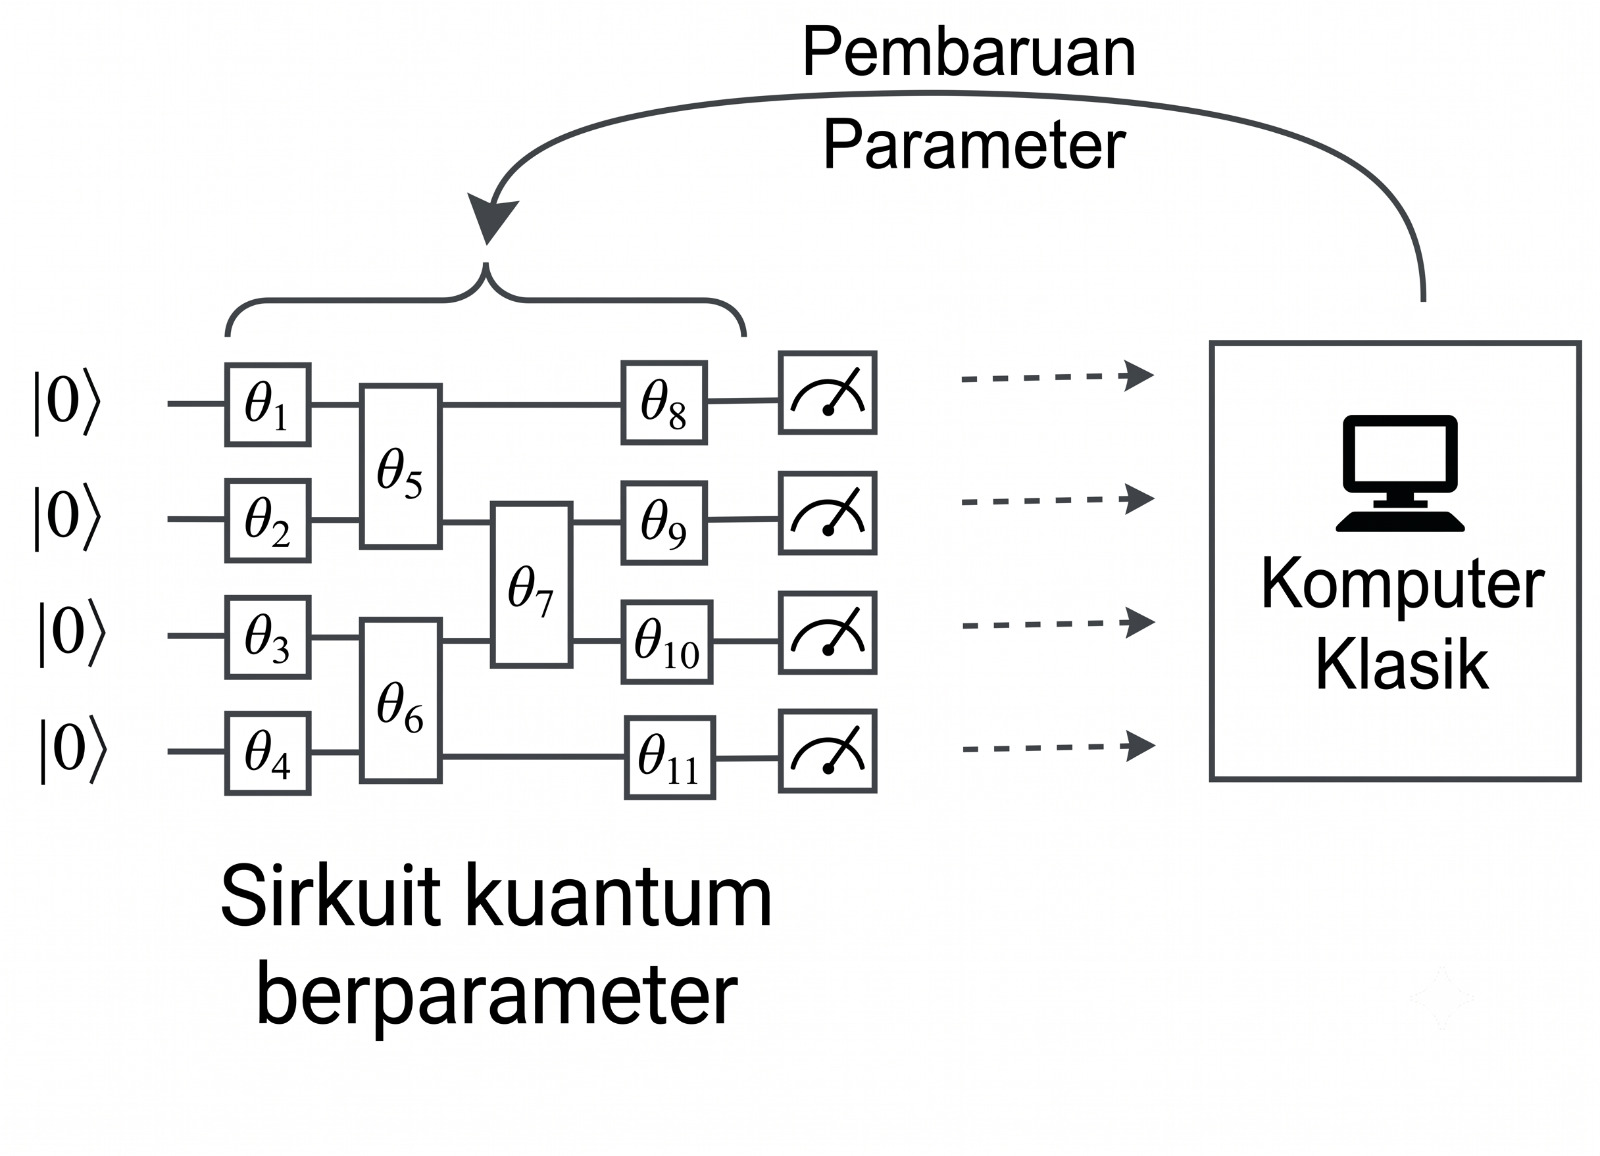
\includegraphics[width=0.4\textwidth]{Gambar/256_PQC1.jpeg} \\
    \end{center}
\end{frame}
